%%%%%%%%%%%%%%%%%%%%%%%%%%%%%%%%%%% SETUP
\documentclass{classes/beamer_GeomaticaUA}
%\documentclass[handout]{Classes/beamer_GeomaticaUA}
\usepackage{styles/beamer_GeomaticaUA}
%\usepackage{styles/Amsterdam}
\usepackage{listings}
\renewcommand{\lstlistlistingname}{Codes}
\renewcommand{\lstlistingname}{Code}


%% LISTING ENVIRONMENTS-----------------------
% Java/c#
\lstnewenvironment{Java}{\lstset{
language=Java,                % choose the language of the code
 frame=Ltbr,
 framerule=0.2pt,
 aboveskip=0.5cm,
 framextopmargin=3pt,
 framexbottommargin=3pt,
 framexleftmargin=0.4cm,
 framesep=0.4pt,
 rulesep=0.4pt,
 %backgroundcolor=\color{white},
 rulesepcolor=\color{gray},
 stringstyle=\ttfamily\color{purple},
 showstringspaces = false,
 %basicstyle=\small\ttfamily,
 commentstyle=\color[rgb]{0.133,0.545,0.133},
 keywordstyle=\color[rgb]{0,0,1},%\bfseries 
 %morekeywords={text,serial,with,owner,to, replace, function, for, if, begin, loop, exit,
 %return,returns,cost,row,volatile,into, setof, double, precision,declare,record,reverse,boolean},
 numbers=left,
 numbersep=14pt,
 breaklines=true
}}{}

% SQL
\lstnewenvironment{SQL}{\lstset{
language=SQL,                % choose the language of the code
 frame=Ltbr,
 framerule=0.2pt,
 aboveskip=0.25cm,
 framextopmargin=3pt,
 framexbottommargin=3pt,
 framexleftmargin=0.4cm,
 framesep=0.4pt,
 rulesep=0.4pt,
 backgroundcolor=\color{white},
 rulesepcolor=\color{gray},
 stringstyle=\ttfamily\color{purple},
 showstringspaces = false,
 basicstyle=\tiny\ttfamily,
 commentstyle=\color[rgb]{0.133,0.545,0.133},
 keywordstyle=\color[rgb]{0,0,1},%\bfseries 
 morekeywords={text,serial,with,owner,to, replace, function, for, if, begin, loop, exit,
 return,returns,cost,row,volatile,into, setof, double, precision,declare,record,reverse,boolean},
 numbers=left,
 numbersep=14pt,
 breaklines=true,
 extendedchars=true,
 literate={á}{{\'a}}1 {é}{{\'e}}1 {í}{{\'i}}1 {ó}{{\'o}}1 {ú}{{\'u}}1 {ñ}{{\~n}}1 {¿}{{?`}}1
}}{}


% Defino un entorno CommandLine Linux
\lstnewenvironment{bash}{\lstset{
language=bash,                % choose the language of the code
 frame=Ltbr,
 framerule=0.2pt,
 aboveskip=0.25cm,
 framextopmargin=3pt,
 framexbottommargin=3pt,
 framexleftmargin=0.4cm,
 framesep=0.4pt,
 rulesep=0.4pt,
 backgroundcolor=\color{white},
 rulesepcolor=\color{gray},
 stringstyle=\ttfamily\color{purple},
 showstringspaces = false,
 basicstyle=\tiny\ttfamily,
 commentstyle=\color[rgb]{0.133,0.545,0.133},
 keywordstyle=\color[rgb]{0,0,1},%\bfseries
 morekeywords={cd,mkdir}
 numbers=left,
 numbersep=14pt,
 breaklines=true,
 extendedchars=true,
 literate={á}{{\'a}}1 {é}{{\'e}}1 {í}{{\'i}}1 {ó}{{\'o}}1 {ú}{{\'u}}1 {ñ}{{\~n}}1 {¿}{{?`}}1
}}{}


% PLR
\lstnewenvironment{PLR}{\lstset{
language=R,                % choose the language of the code
 frame=Ltbr,
 framerule=0.2pt,
 aboveskip=0.5cm,
 framextopmargin=3pt,
 framexbottommargin=3pt,
 framexleftmargin=0.4cm,
 framesep=0.4pt,
 rulesep=0.4pt,
 %backgroundcolor=\color{white},
 rulesepcolor=\color{gray},
 stringstyle=\ttfamily\color{purple},
 showstringspaces = false,
 %basicstyle=\small\ttfamily,
 commentstyle=\color[rgb]{0.133,0.545,0.133},
 keywordstyle=\color[rgb]{0,0,1},%\bfseries 
 morekeywords={text,serial,with,owner,to, replace, function, for, if, begin, loop, exit,
 return,returns,cost,row,volatile,into, setof, double, precision,declare,record,reverse},
 numbers=left,
 numbersep=14pt,
 breaklines=true
}}{}

% R
\lstnewenvironment{R}{\lstset{
language=R,                % choose the language of the code
 frame=Ltbr,
 framerule=0.2pt,
 aboveskip=0.5cm,
 framextopmargin=3pt,
 framexbottommargin=3pt,
 framexleftmargin=0.4cm,
 framesep=0.4pt,
 rulesep=0.4pt,
 %backgroundcolor=\color{white},
 rulesepcolor=\color{gray},
 stringstyle=\ttfamily\color{purple},
 showstringspaces = false,
 alsoother={:_\$},
 %basicstyle=\small\ttfamily,
 commentstyle=\color[rgb]{0.133,0.545,0.133},
 keywordstyle=\color[rgb]{0,0,1},%\bfseries 
 %morekeywords={text,serial,with,owner,to, replace, function, for, if, begin, loop, exit,
 %return,returns,cost,row,volatile,into, setof, double, precision,declare,record,reverse},
 numbers=left,
 numbersep=14pt,
 breaklines=true
}}{}

% PHP
\lstnewenvironment{PHP}{\lstset{
language=PHP,                % choose the language of the code
 frame=Ltbr,
 framerule=0.2pt,
 aboveskip=0.5cm,
 framextopmargin=3pt,
 framexbottommargin=3pt,
 framexleftmargin=0.4cm,
 framesep=0.4pt,
 rulesep=0.4pt,
 %backgroundcolor=\color{white},
 rulesepcolor=\color{gray},
 stringstyle=\ttfamily\color{purple},
 showstringspaces = false,
 %basicstyle=\small\ttfamily,
 commentstyle=\color[rgb]{0.133,0.545,0.133},
 keywordstyle=\color[rgb]{0,0,1},%\bfseries 
 numbers=left,
 numbersep=14pt,
 breaklines=true
}}{}

% Diagramas entidad relación
% Ver ejemplo en http://heisenbugs.blogspot.com.es/2010/10/making-great-er-diagrams-without.html
\usepackage{styles/tikz-er2}
\usetikzlibrary{positioning}
\usetikzlibrary{shadows}
\usetikzlibrary{mindmap}
% Diagramas UML
% Ver http://perso.ensta-paristech.fr/~kielbasi/tikzuml/index.php?lang=en
\usepackage{styles/tikz-uml}

%% ER styles
\tikzstyle{every entity} = [top color=white, bottom color=blue!30,
draw=blue!50!black!100, drop shadow]
\tikzstyle{every weak entity} = [drop shadow={shadow xshift=.7ex,
shadow yshift=-.7ex}]
\tikzstyle{every attribute} = [top color=white, bottom color=yellow!20,
draw=yellow, node distance=7em, drop shadow]
\tikzstyle{every relationship} = [top color=white, bottom color=red!20,
draw=red!50!black!100, drop shadow]
\tikzstyle{every isa} = [top color=white, bottom color=green!20,
draw=green!50!black!100, drop shadow]


%% Árboles de directorios
%\usepackage{tikz}
%\usetikzlibrary{trees}

%\tikzstyle{every node}=[draw=black,thick,anchor=west]
%\tikzstyle{selected}=[draw=red,fill=red!30]
%\tikzstyle{optional}=[dashed,fill=gray!50]

%%%%%%%%%%%%%%%%%%%%%%%%%%%%%%%%%%%
%\begin{frame}{Modelo Jerárquico}
%\begin{columns}
%\begin{column}{0.5\textwidth}
%\begin{center}

%\begin{tikzpicture}[%
%  grow via three points={one child at (0.5,-0.7) and
%  two children at (0.5,-0.7) and (0.5,-1.4)},
%  edge from parent path={(\tikzparentnode.south) |- (\tikzchildnode.west)}]
%  \node {País}
%    child { node {Prov A}}		
%    child { node [selected] {Prov C}
%      child { node {Muni C1}}
%      child { node [selected]{Muni C2}
%      	child { node [selected] {Parc 1}}
%      	child { node [selected] {Parc2}}
%      	child { node [selected] {Parc n}}
%      }
%      child [missing] {}	
%      child [missing] {}				
%	  child [missing] {}	
%      child { node [optional] {Muni C$n$}}
%    }
%    child [missing] {}				
%    child [missing] {}	
%    child [missing] {}				
%    child [missing] {}	
%    child [missing] {}							
%    child [missing] {}				
%    child { node [optional] {Prov $n$}};
%\end{tikzpicture}
%\end{center}
%\end{column}
%
%\begin{column}{0.5\textwidth}
%El modelo jerárquico organiza los datos en una estructura ramificada (\textit{tree structure}).\\[3ex]
%
%\textbf{Consulta:}\\
%Cultivos/superficie en el municipio C2\\[3ex]
%
%\textbf{Coste:} \\
%Una búsqueda por Prov, otra por Muni de la Prov C y calculamos las estadísticas para todos. No hay que seguir buscando.
%\end{column}
%\end{columns}
%\end{frame}

%%%%%%%%%%%%%%%%%%%%%%%%%%%%%%%%%%% METADATA
\author{Miguel Fernández Moreno}
\title{PostGIS (II)}
\titlegraphic{
\includegraphics[height=0.6cm]{logos/logo_ua.png} \hspace{1cm} 
\includegraphics[height=1cm]{logos/iig}} 
\institute[GeomaticaLab]{Instituto Interuniversitario de Geografía\\Laboratorio de Geomática} 
\date{13 de noviembre de 2014}
\subject{Cuarta sesión del curso ``Diseño, creación y gestión de Bases de Datos Geográficas con PostGIS''}


%%%%%%%%%%%%%%%%%%%%%%%%%%%%%%%%%%% SLIDES
\begin{document}

\begin{frame}
\titlepage
\end{frame}

\section[Introducción]{Presentación y comentarios}
\subsection{Descripción general del SQL}
\begin{frame}{¿Que vamos a hacer hoy?}
\begin{enumerate}
\item Índices espaciales
\item Topología
\item Geoprocesamiento
\end{enumerate}
\end{frame}


\section[Índices]{Índices espaciales}
%%SQL entre otros lenguajes

%%%%%%%%%%%%%%%%%%%%%%%%%%%%%%%%%%%
\begin{frame}[fragile]
\frametitle{El índice en una base de datos}
Estructura de datos que mejora la velocidad de las operaciones, por medio de un identificador único de cada fila de una tabla, permitiendo un rápido acceso a los registros de una tabla en una base de datos. 
\end{frame}

\begin{frame}[fragile]
\frametitle{¿Por qué usarlos?}
\begin{itemize}
\item Evitamos un lectura completa de la tabla
\item Rápidez en la ejecución de las consultas
\item Evitamos sobrecarga de CPU, sobrecarga de disco y concurrencia
\item Es una ventaja en tablas con gran cantidad de datos
\end{itemize}
\end{frame}

% --------------------------------------------------- Slide --
\begin{frame}[fragile]
\frametitle{Índices PostgreSQL / Postgis}
\begin{description}
\item[B-Trees]\hfill \\ Se usa para datos que pueden ser ordenados sobre un eje: números, letras, fechas. No es aplicable a los datos GIS.
\item[R-Trees] \hfill \\Divide los datos en rectángulos, sub-rectángulos, sub-sub-rectángulos, etc.
\item[GiST] \hfill \\Parte los datos \emph{cosas que están a un lado}, \emph{cosas que se superponen}, \emph{cosas que están dentro}. PostGIS utiliza un índice R-Tree implementado en la parte superior de GiST para indexar los datos GIS.
\end{description}
\end{frame}
% --------------------------------------------------- Slide --
\begin{frame}[fragile]
\frametitle{Crear índice usando GiST}
\lstset{caption=Ejemplo de índice GiST,label=sql:gist}
\begin{SQL}
-- La sintaxis para crear un índice GiST en la columna geometría:
CREATE INDEX index_ua_pc2 ON ua_pc2 USING GIST (geom);
\end{SQL}

\end{frame}
% --------------------------------------------------- Slide --
\begin{frame}[fragile]
\frametitle{GiST}
\lstset{caption=Comprobar velocidad del índice GiST,label=sql:qIndex}
\begin{SQL}
-- Sintaxis para comprobar el funcionamiento del índice:
SELECT codigo ,avg(z) AS media FROM estancias, ua_pc2
WHERE st_intersects(estancias.geom, ua_pc2.geom) 
GROUP BY codigo;
\end{SQL}

\end{frame}
% --------------------------------------------------- Slide --
\begin{frame}[fragile]
\frametitle{Funcionamiento de la consulta con el índice}
\begin{block}{Resultado sin índice}
\center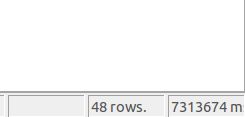
\includegraphics[scale=0.5]{images/resultWithoutIndex.png}
\end{block}
\begin{block}{Resultado con índice}
\center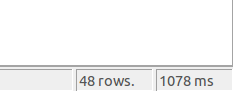
\includegraphics[scale=0.5]{images/resultWithIndex.png}
\end{block}
\end{frame}
% --------------------------------------------------- Slide --
\begin{frame}[fragile]
\frametitle{Funcionamiento de la consulta con el índice}
\center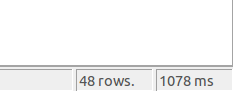
\includegraphics[scale=0.5]{images/resultWithIndex.png}
\end{frame}
% --------------------------------------------------- Slide --
\section[Operadores]{Operadores espaciales}
%%%%%%%%%%%%%%%%%%%%%%%%%%%%%%%%%%%
\begin{frame}[fragile]
\frametitle{Operadores espaciales (I)}
\begin{description}
\item[\&\&]Devuelve TRUE si la bounding box de la geometría A intersecta con la bounding box de la geometría B.
\item[\&$<$]Devuelve TRUE if A's bounding box overlaps or is to the left of B's.
\item[\&$<|$]Devuelve TRUE if A's bounding box overlaps or is below B's.
\item[\&$>$]Devuelve TRUE if A' bounding box overlaps or is to the right of B's.
\item[$<<$]Devuelve TRUE if A's bounding box is strictly to the left of B's.
\item[$<<|$]Devuelve TRUE if A's bounding box is strictly below B's.
\end{description}
\end{frame}
%%%%%%%%%%%%%%%%%%%%%%%%%%%%%%%%%%%
\begin{frame}[fragile]
\frametitle{Operadores espaciales (II)}
\begin{description}
\item[=]Devuelve TRUE if A's bounding box is the same as B's. Uses double precision bounding box.
\item[$>>$]Devuelve TRUE if A's bounding box is strictly to the right of B's.
\item[$@$]Devuelve TRUE if A's bounding box is contained by B's.
\item[$\mid$\&$>$]Devuelve TRUE if A's bounding box overlaps or is above B's.
\item[$\mid\gg$]Devuelve TRUE if A's bounding box is strictly above B's.
\item[$\thicksim$]Devuelve TRUE if A's bounding box contains B's.
\end{description}
\end{frame}
%%%%%%%%%%%%%%%%%%%%%%%%%%%%%%%%%%%
\begin{frame}[fragile]
\frametitle{Operadores espaciales (III)}
\begin{description}
\item[$~=$]Devuelve TRUE if A's bounding box is the same as B's.
\item[$<->$]Devuelve la distancia entre dos puntos. For point / point checks it uses floating point accuracy (as opposed to the double precision accuracy of the underlying point geometry). For other geometry types the distance between the floating point bounding box centroids is returned. Useful for doing distance ordering and nearest neighbor limits using KNN gist functionality.
\item[$<\#>$]Devuelve la distancia entre la bounding box de dos geometrías. For point / point checks it's almost the same as distance (though may be different since the bounding box is at floating point accuracy and geometries are double precision). Useful for doing distance ordering and nearest neighbor limits using KNN gist functionality.
\end{description}
\end{frame}
\section[Ejercicios]{Operadores espaciales}
% --------------------------------------------------- Slide --

% --------------------------------------------------- Slide --


\end{document}
